\chapter{MIMD Architectures}
In a distributed memory MIMD machine, the processor/memory pairs are replicated and are then connected via an interconnection network. In a shared memory MIMD machine, the processors and memories are replicated independently and are then connected via an interconnection network.

MIMD machines can be classified into a hierarchy, as can be seen in \autoref{fig:screenshot115}.

\begin{figure}
\centering
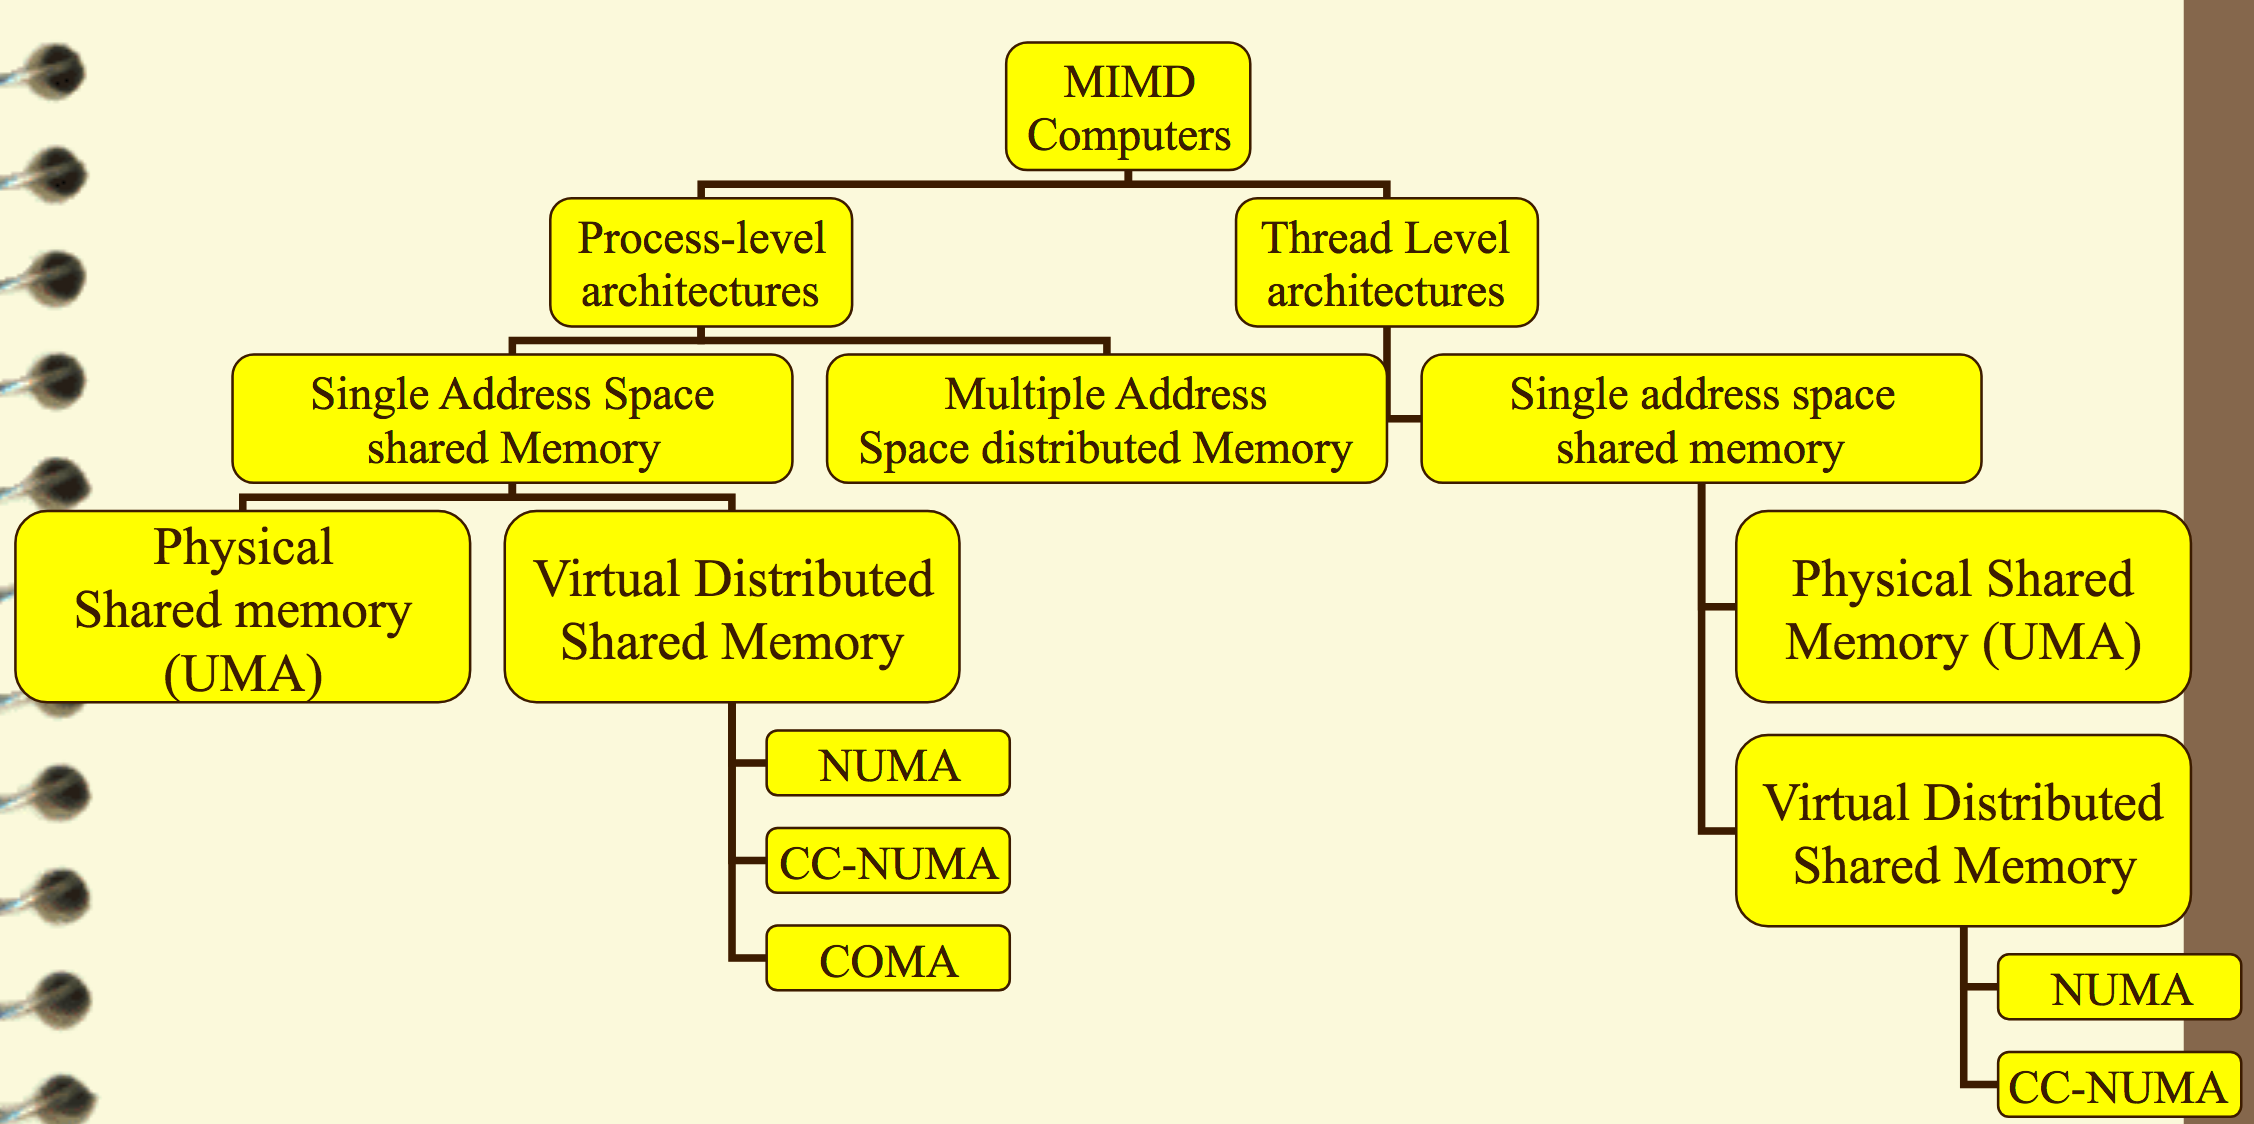
\includegraphics[width=0.7\linewidth]{screenshot115}
\caption{Classification of MIMD computers.}
\label{fig:screenshot115}
\end{figure}

\section{Distributed Memory}
\begin{figure}
\centering
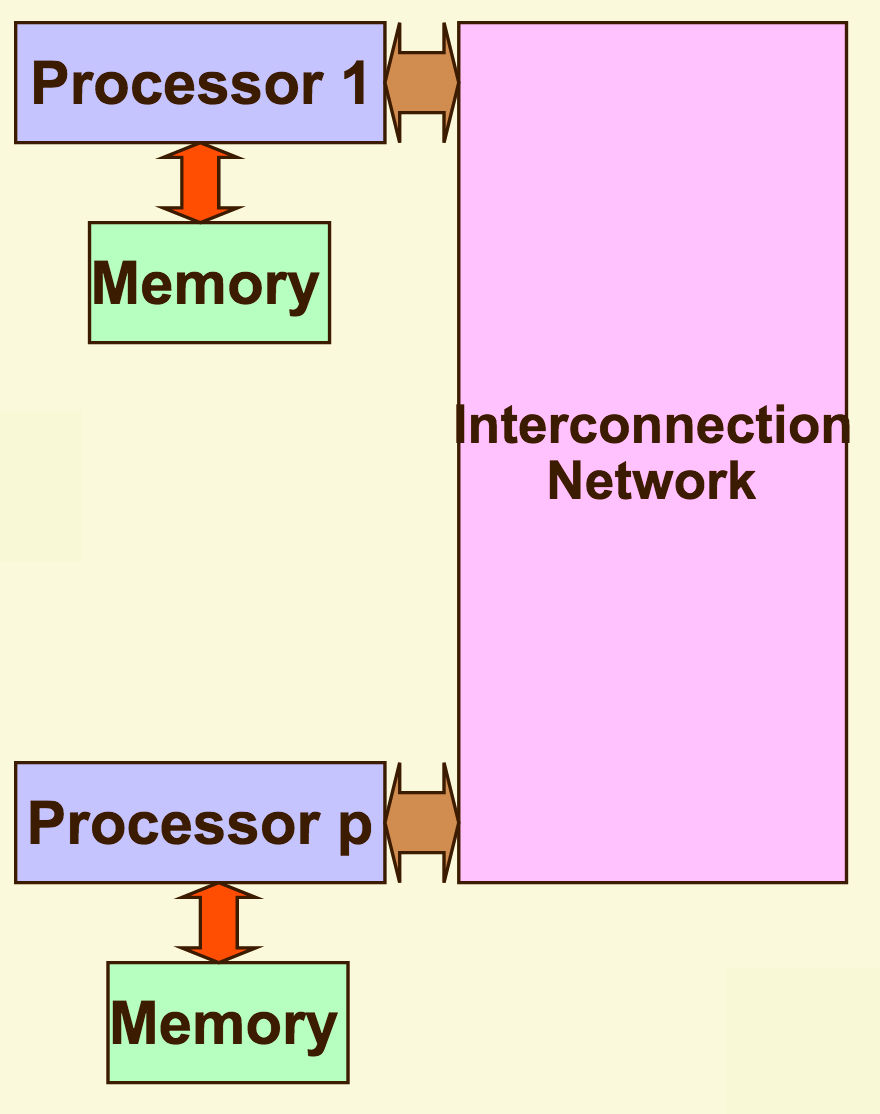
\includegraphics[width=0.7\linewidth]{screenshot110}
\caption{Distributed memory system.}
\label{fig:screenshot110}
\end{figure}

In a distributed memory system, each processor has its own local memory that is not shared with other processors (\autoref{fig:screenshot110}). The access to this local memory module is much faster than remote memory. The hardware accesses remote memory through load/store primitives and a message passing layer. Cache memory is also used for local memory traffic. Messages can be memory-memory or cache-cache.

Distributed memory offers the following advantages: \begin{itemize}
\item Local memory traffic offers less contention than in shared memory.
\item Highly scalable.
\item Sophisticated synchronization features like monitors or semaphores are not needed. Message passing serves the dual purposes of data transmission and synchronisation.
\end{itemize}

However, it is subject to the following disadvantages: \begin{itemize}
\item Load balancing is difficult.
\item Message passing can lead to synchronisation failures, including deadlock (i.e. the sequence of BlockingSend $\rightarrow$ BlockingReceive, BlockingReceive $\rightarrow$ BlockingSend can occur).
\item Entire data structures need to be copied, which can be an intensive process.
\item The overhead for small messages is high relative to the size of the message.
\end{itemize}

\section{Shared Memory}
\begin{figure}
\centering
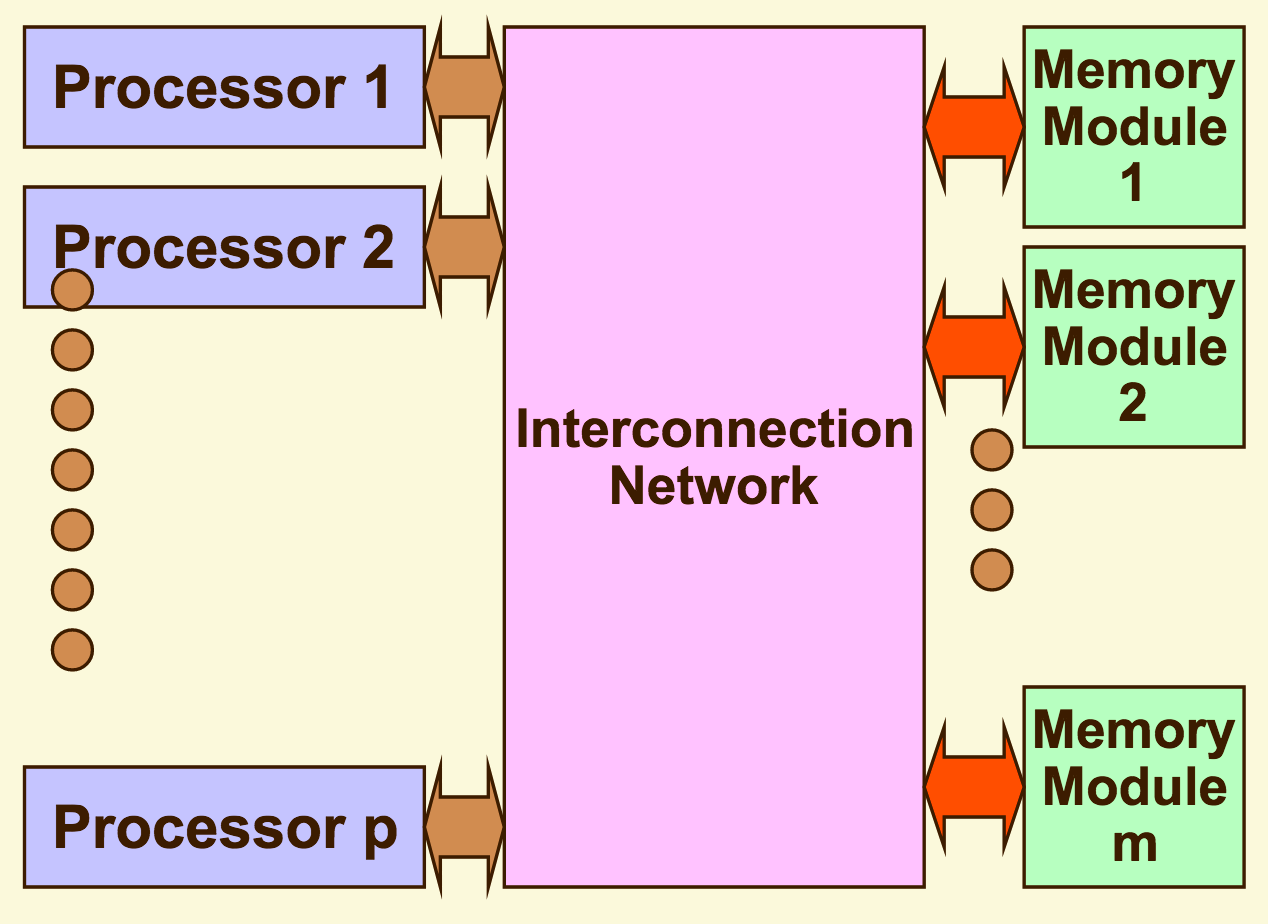
\includegraphics[width=0.7\linewidth]{screenshot111}
\caption{Shared memory system.}
\label{fig:screenshot111}
\end{figure}

In a shared memory system, all processors have equal access to shared memory modules (\autoref{fig:screenshot111}). Local caches reduce memory traffic, network traffic, and memory access time. As memory is synchronised between the processes, load/store is indivisible.

Shared memory offers the following advantages: \begin{itemize}
\item There is no need to partition code or data; the system handles this automatically.
\item There is no need to move data explicitly.
\item Existing programming languages and/or compilers can be used.
\end{itemize}

However, it is subject to the following disadvantages: \begin{itemize}
\item Synchronisation of resources is difficult.
\item Lack of scalability; IPC \footnote{I assume this is interprocess communication, but it could also be instructions-per-clock. Overloaded acronyms are \textit{fun!}} becomes a bottleneck. This can be addressed by using a high-throughput and low-latency network, using cache memory (but this will lead to cache coherence issues), or using a distributed shared memory architecture.
\end{itemize}

\section{Distributed Shared Memory}
There are three choices for design that can be made: \begin{itemize}
\item Non-uniform memory access (NUMA, \autoref{fig:screenshot112}): Cray T3D
\item Cache-coherent non-uniform memory access (CC-NUMA, \autoref{fig:screenshot113}): Convex SPP, Stanford DASH
\item Cache-only memory access (COMA, \autoref{fig:screenshot114}): KSR-1
\end{itemize}

\begin{figure}
\centering
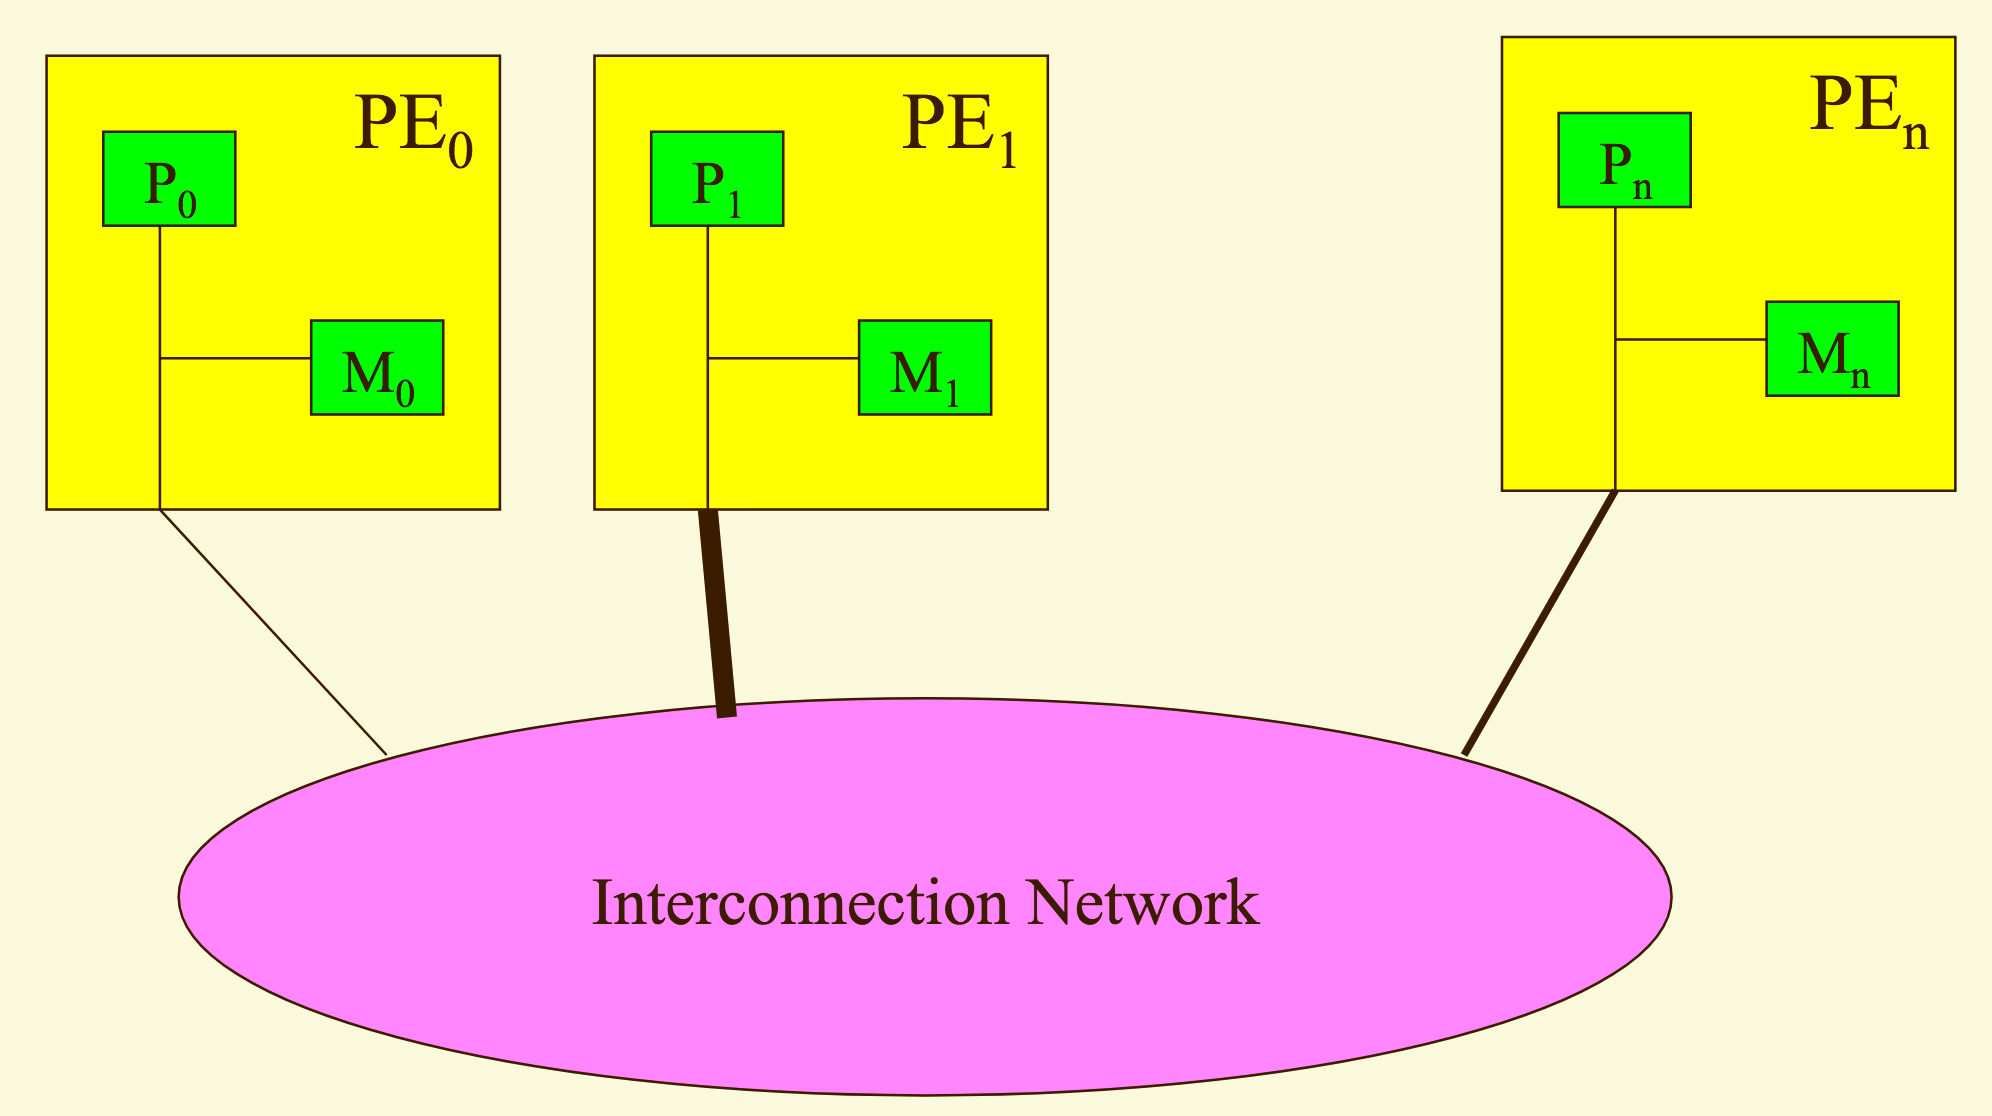
\includegraphics[width=0.7\linewidth]{screenshot112}
\caption{NUMA.}
\label{fig:screenshot112}
\end{figure}

\begin{figure}
\centering
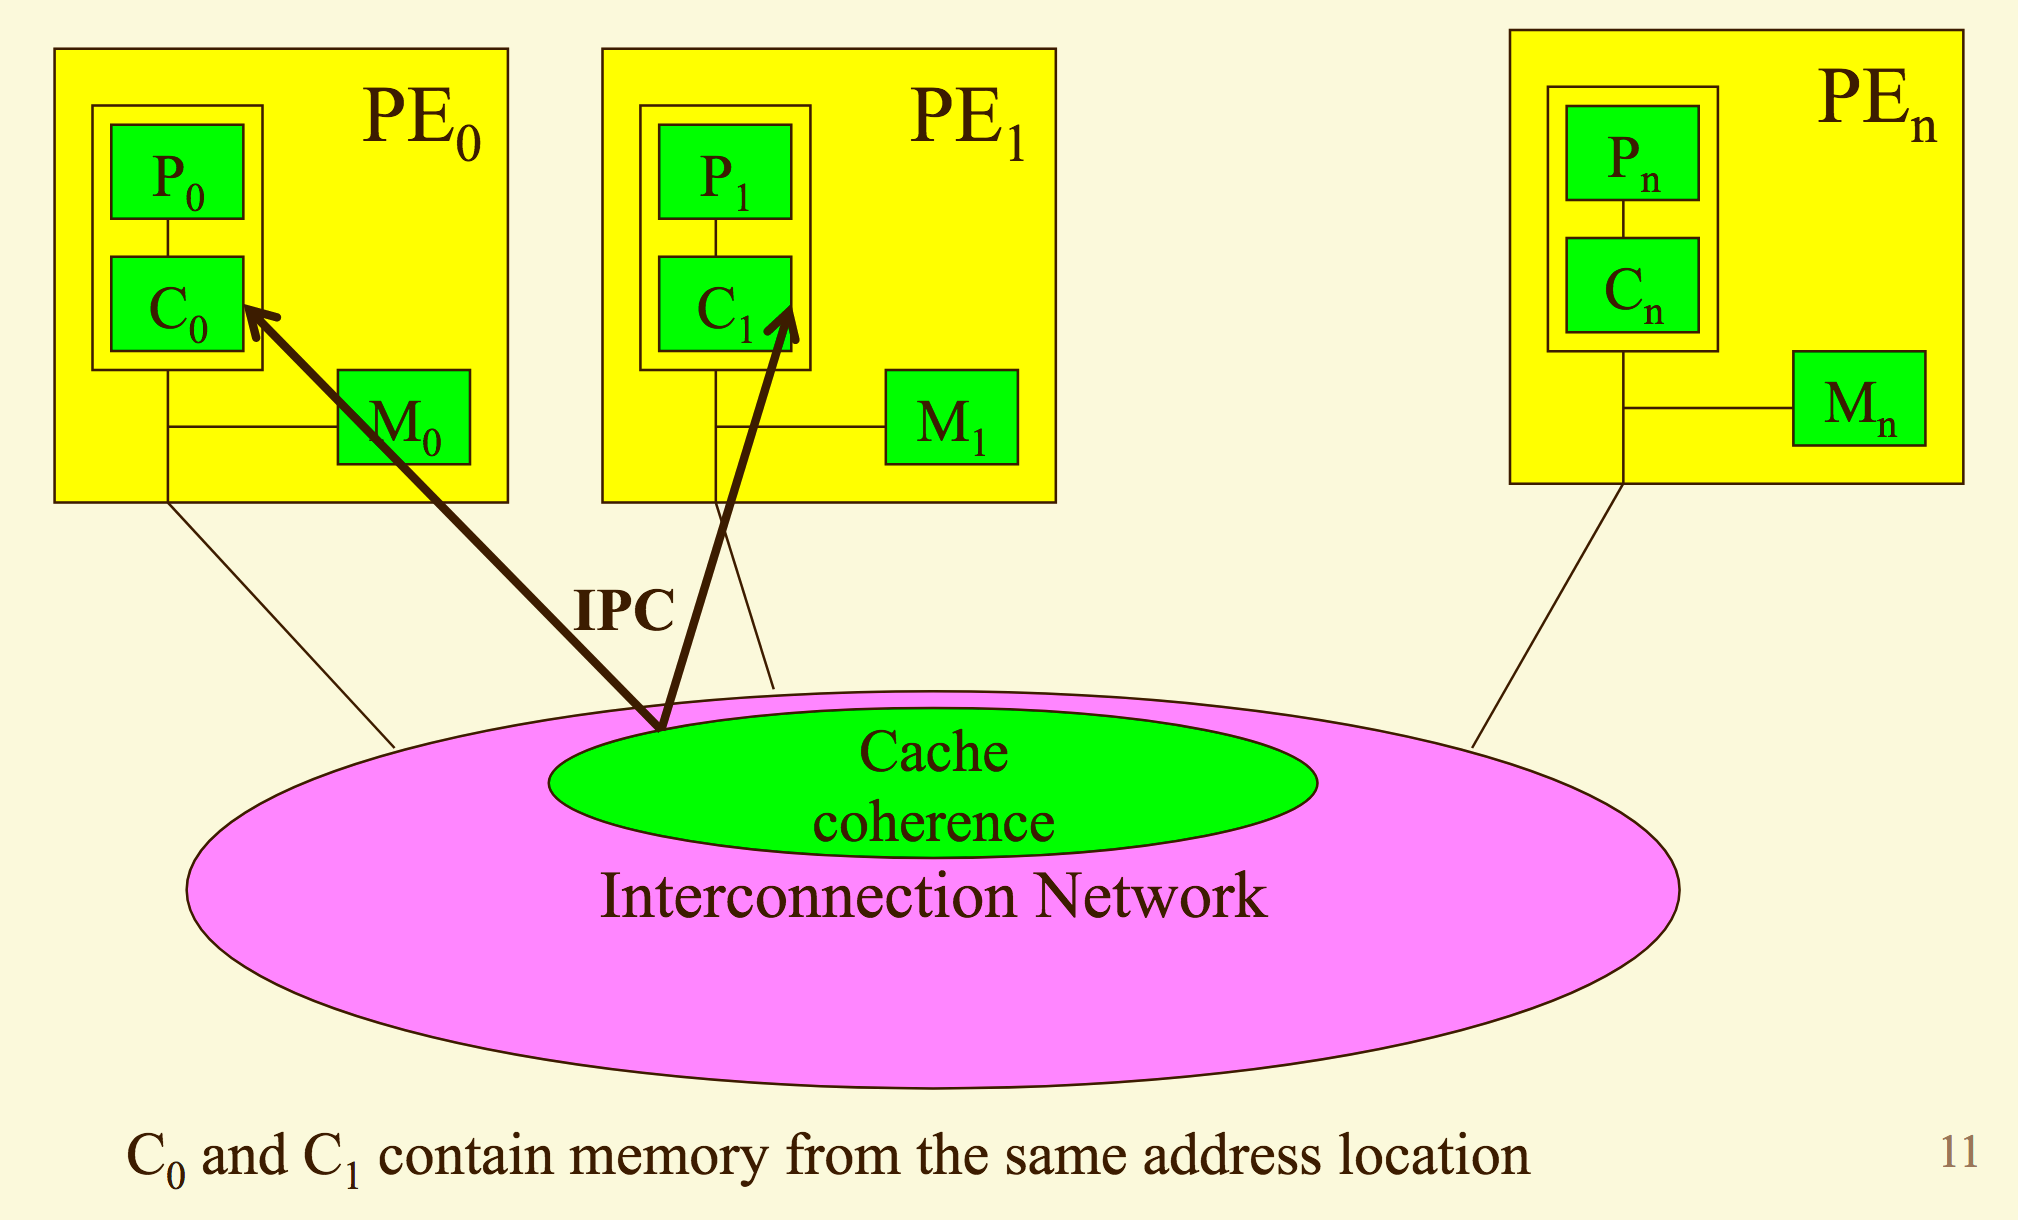
\includegraphics[width=0.7\linewidth]{screenshot113}
\caption{CC-NUMA.}
\label{fig:screenshot113}
\end{figure}

\begin{figure}
\centering
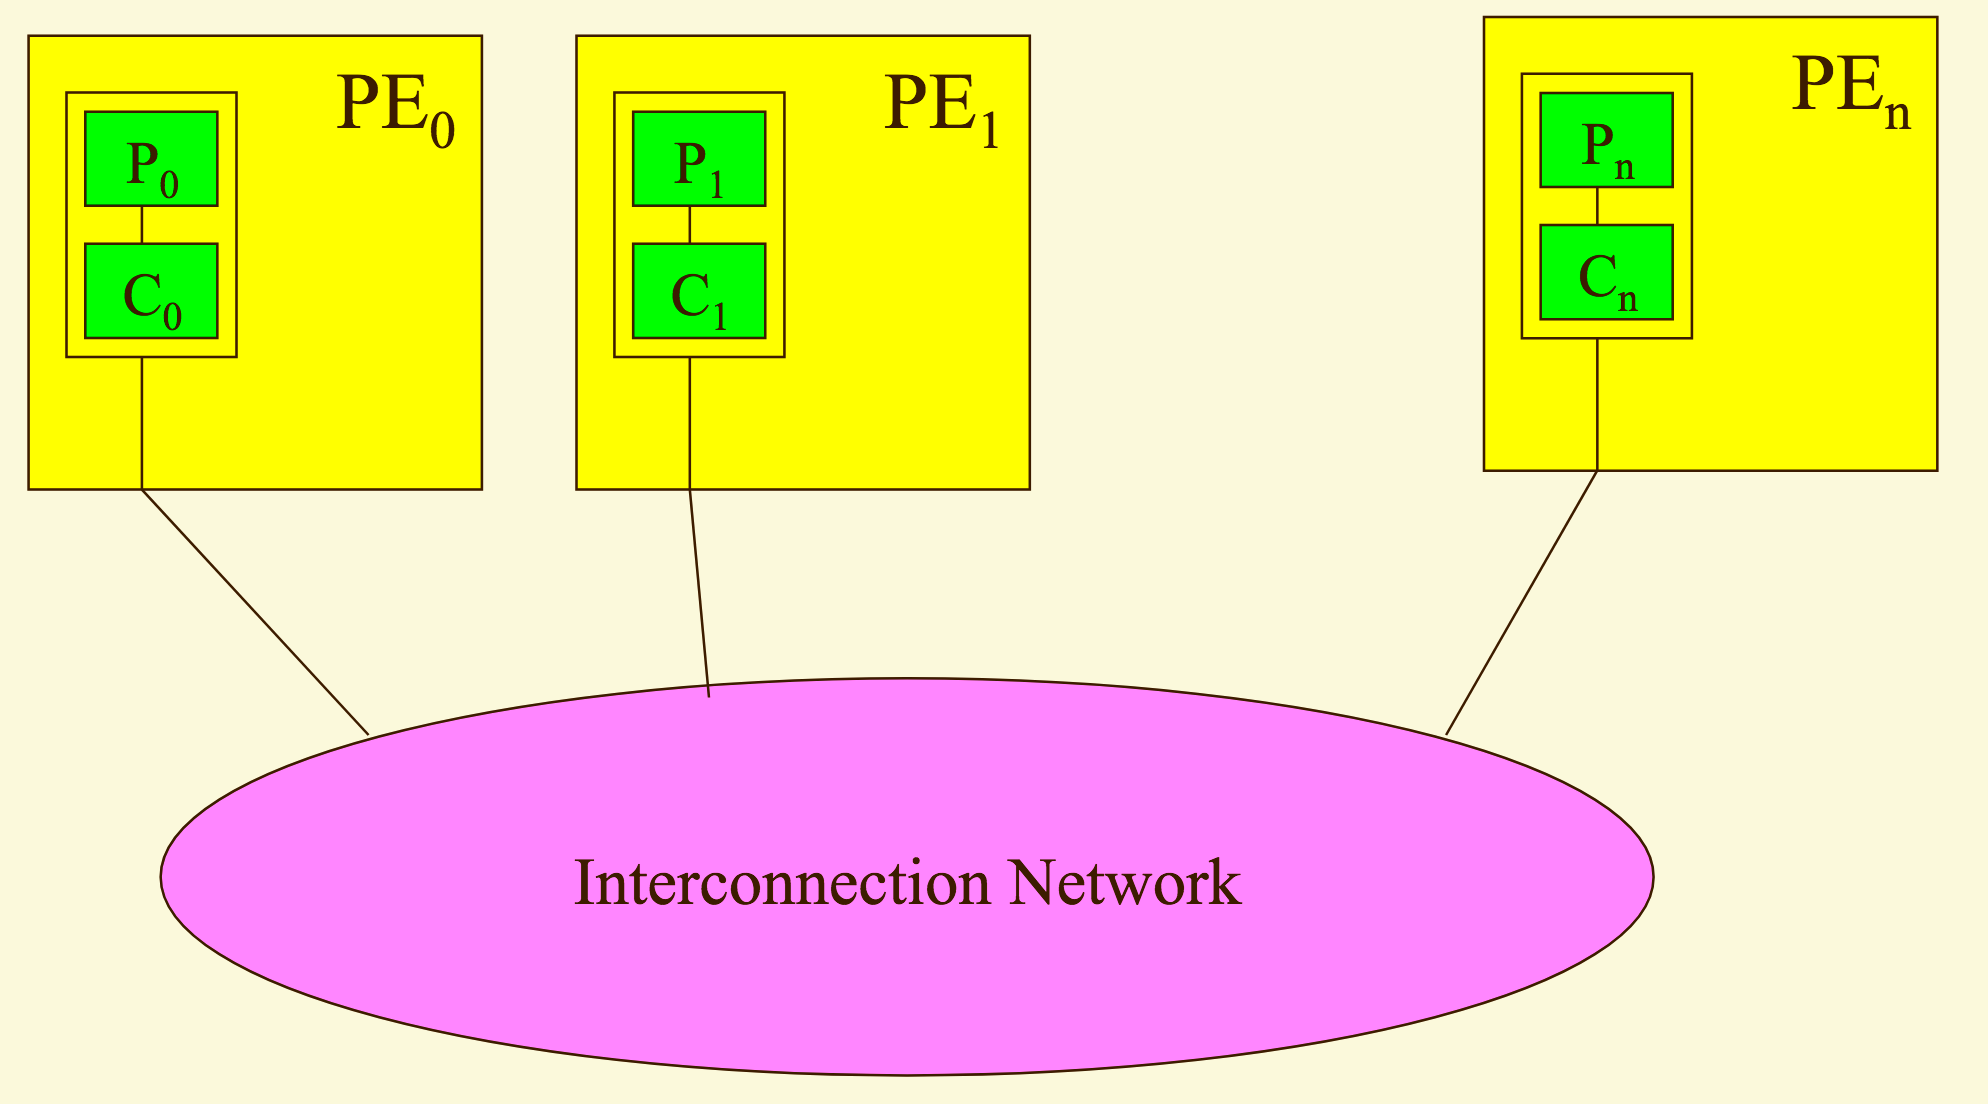
\includegraphics[width=0.7\linewidth]{screenshot114}
\caption{COMA.}
\label{fig:screenshot114}
\end{figure}

\section{Problems of Scalable Computers}
A scalable computer needs to be able to tolerate and hide the latency of remote loads, as shown in \autoref{fig:screenshot116}; this is made worse if the output of one computation relies on another to complete.

\begin{figure}
\centering
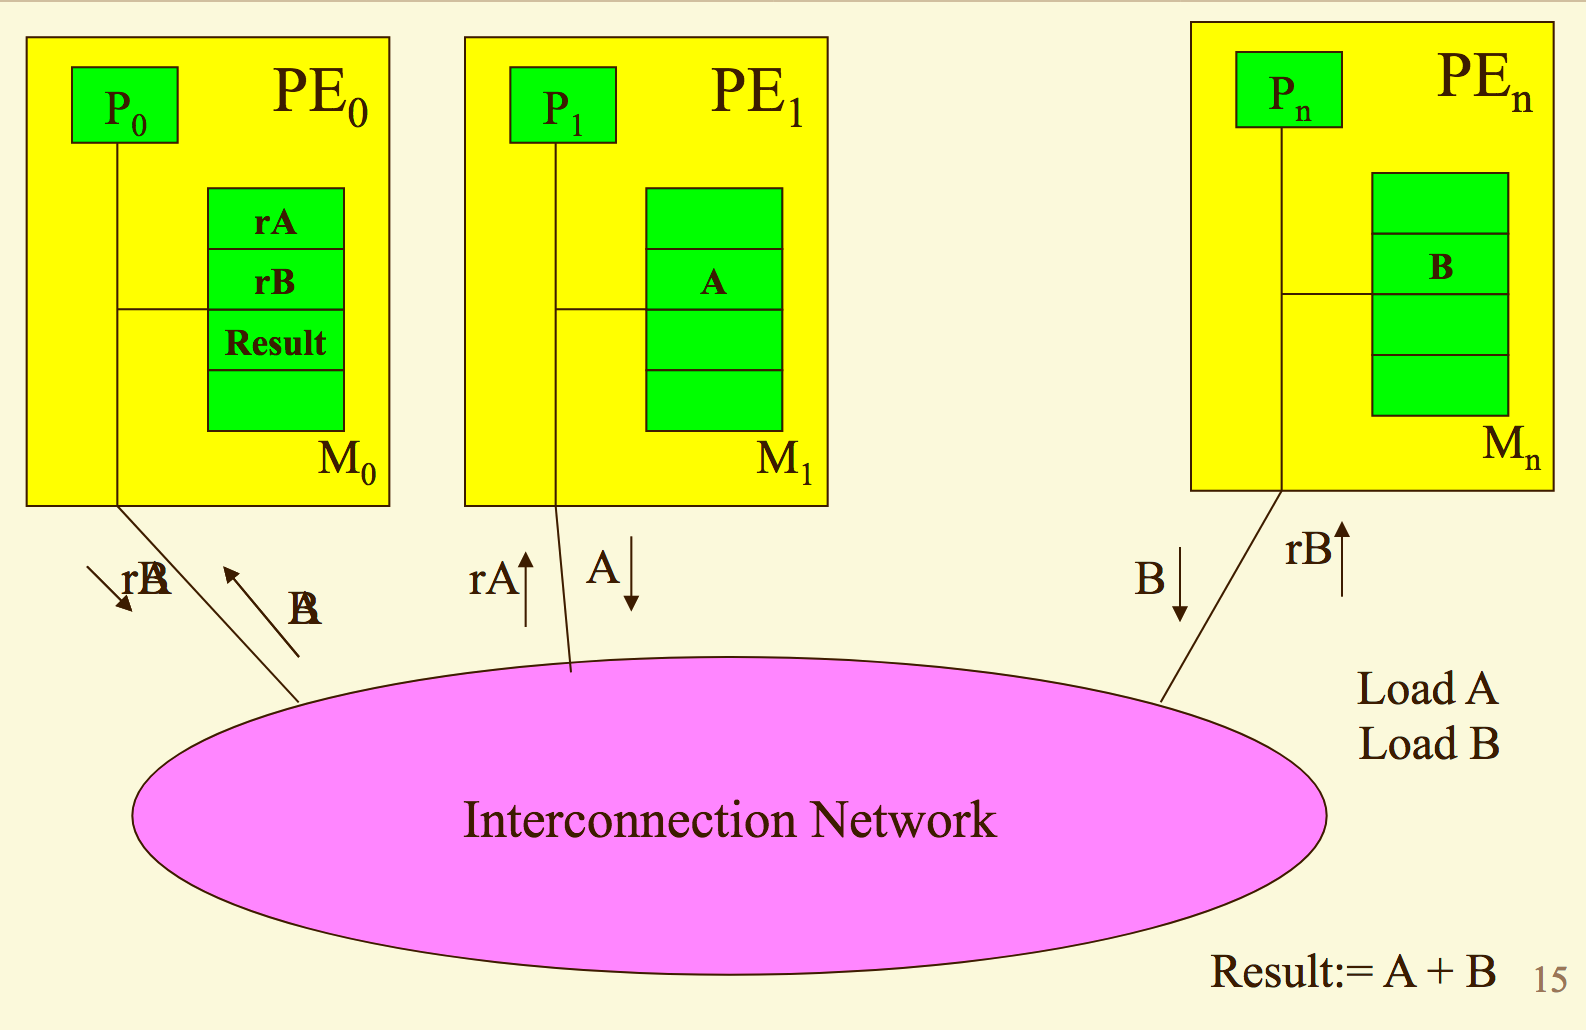
\includegraphics[width=0.7\linewidth]{screenshot116}
\caption{Tolerating remote loads.}
\label{fig:screenshot116}
\end{figure}

It also needs to be able to tolerate and hide idling brought about by synchronisation among processors.

To tolerate latency, a variety of techniques can be used: \begin{itemize}
\item \textbf{Cache memory}: Maintaining local copies of remote memory that is cheap to access. This lowers the cost of remote access, but introduces the cache coherence problem.
\item \textbf{Prefetching}: Prefetching relevant data before it is needed. This is already present to some extent, so the cost of implementation is low. However, it will increase network load.
\item \textbf{Threads + fast context switching}: Using local multithreading to minimise the time spent idling. This is acceptance that a remote action will take a long time, and using this time effectively to cover the overhead.
\end{itemize}
However, these solutions do not solve synchronisation issues; latency-tolerant algorithms must be used fo rthat.

\section{Design issues of scalable MIMD}
Scalable MIMD is subject to several design issues that need to be considered.

The processor design must consider pipelining and issues that arise from running instructions in parallel. In doing so, concerns with atomic data access, prefetching, cache memory, message passing and more may be raised.

The interconnection network design must be designed to be scalable, high-bandwidth and low-latency.

Memory in the system may become a complex subject if a shared memory design is used. For performance, the shared memory will need local caches on each processor. However, maintaining these caches and keeping them up to date with the remote memory results in the \textit{cache coherency} problem, in which the cache may desynchronise and cause issue.

Finally, the I/O subsystem needs to be designed to handle parallel I/O. A parallel system that cannot actually receive or submit data quickly enough will be bottlenecked.